\section{Implementation}\label{a:impl}

\paragraph{Channel.} A \Digitiser{} oscilloscope digitises the probe at \DigBits{}~bits
and streams the raw samples at \Fs{}~S/s. No filter precedes the converter, so current
variance above the Nyquist frequency folds into the band. We bound it from bursts
recorded at \BurstRate{}~MS/s, assuming no rejection. Under training the folded
variance is at most \AliasTrainPct\% of the in-band variance. Under idle, where the
current is small, it is at most \AliasIdleX{} times the in-band variance. At this bound,
both the raw-spectrum and the envelope features of idle windows would mostly describe
folded variance. Idle windows help set each detector's $\tau_\alpha$ and fit $s_R$, so a
different digitiser or an anti-alias filter could move them; we did not test this. The
low rate costs little signal. In the same bursts, \ChainBelowBand\% of a training trace's variance lies below
\ChainBandKhz{}~kHz, and the envelope at our rate matches one sampled ten times faster
to within \ChainEnvPct\%.

\paragraph{Corpus.} \Cref{t:corpus} counts runs, hours and windows per workload and
split.

\begin{table}[!htbp]
  \centering
  \small
  % generated by scripts/table_corpus.py from results/windows/manifest.json (repo_commit 018c3a2, corpus_commit 73ffebe)
% runs, scored hours and 5 s-hop windows per workload and split
\begin{tabular}{lrrrrrrrrr}
\toprule
 & \multicolumn{3}{c}{$\mathcal{D}_{\mathrm{dev}}$} & \multicolumn{3}{c}{$\mathcal{D}_{\mathrm{test}}$} & \multicolumn{3}{c}{$\mathcal{D}_{\mathrm{cal}}$} \\
\cmidrule(lr){2-4}\cmidrule(lr){5-7}\cmidrule(lr){8-10}
Workload & runs & h & windows & runs & h & windows & runs & h & windows \\
\midrule
honest training & 14 & 4.06 & 2905 & 4 & 0.95 & 680 & 2 & 0.48 & 340 \\
time-sharing & 3 & 0.71 & 510 & 7 & 2.22 & 1586 & -- & -- & -- \\
co-location & 3 & 0.72 & 510 & -- & -- & -- & -- & -- & -- \\
jitter & 4 & 0.95 & 678 & -- & -- & -- & -- & -- & -- \\
padding & 1 & 0.24 & 170 & -- & -- & -- & -- & -- & -- \\
power cap & 2 & 0.48 & 340 & -- & -- & -- & -- & -- & -- \\
declared decode & 2 & 0.48 & 340 & 2 & 0.48 & 340 & 1 & 0.24 & 170 \\
declared prefill & 1 & 0.24 & 170 & -- & -- & -- & -- & -- & -- \\
declared idle & 1 & 0.24 & 170 & 4 & 8.35 & 5994 & 1 & 0.24 & 170 \\
non-AI work & 4 & 0.95 & 681 & 4 & 0.95 & 680 & 2 & 0.48 & 340 \\
\midrule
total & 35 & 9.06 & 6474 & 21 & 12.94 & 9280 & 6 & 1.43 & 1020 \\
\bottomrule
\end{tabular}

  \caption{The corpus per workload and split: runs, scored hours and windows at the
    window-level hop. Time-sharing on the test day is the embedded episodes of
    \cref{s:works}.}
  \label{t:corpus}
\end{table}

\paragraph{Detectors.} The classifier's two stages are random forests and the
signature check is an isolation forest, all from scikit-learn with \ForestTrees{} trees,
default settings otherwise and a fixed seed.

\paragraph{Intervals.} For one run, a circular block bootstrap resamples blocks of
\BootBlock{} consecutive windows (\BootBlockS~s), \NBoot{} times
(\NBootBound{} for the episode lower bounds and the equivalence test). For two runs it
resamples within each run and pools. For three or more it resamples runs. Thresholds
stay fixed in every resample. On the monitor, the upper bound on $F$ assumes Poisson
onsets; the interval on $A$ resamples blocks of \OnsetBlockMin~min. An episode lower bound
is the smaller of a one-sided Clopper--Pearson bound and a block bootstrap over blocks
of \EpBlock{} consecutive episodes.

\paragraph{Episodes.} An episode that starts while an alarm is active counts as
detected only where the run's flag rate on gap windows, which hold no training, is at
most \GapGuard; we call this the gap guard. A run whose gaps hold no whole window takes the pooled gap flag rate
of the other runs. Otherwise only new onsets count, and the result is marked
onset-only. The delay $D$ is taken over episodes that raise a new alarm.
Under the complete reference, \EpPreRone{} of the \EpScored{} scored episodes start in alarm, and all are
credited (\cref{t:t7}).

\paragraph{Data and code.} The corpus is archived on Zenodo
\citep{kimpson2026corpus}. The analysis code, every committed result, and the scripts
that make every figure, table and number in this paper are at
\url{https://github.com/tomkimpson/verifying-declared-ai-workloads}. The window
features are not stored there; \texttt{scripts/make\_windows.py} regenerates them from
the archive. Every result
was computed against corpus commit \texttt{\CorpusCommit}.

\FloatBarrier
\section{The reference changes in detail}\label{a:reference}

\paragraph{Scores.} \Cref{f:f7} shows the per-window scores behind the complete
reference and the decode-only fit of \cref{t:t7}.

\begin{figure}[!htbp]
  \centering
  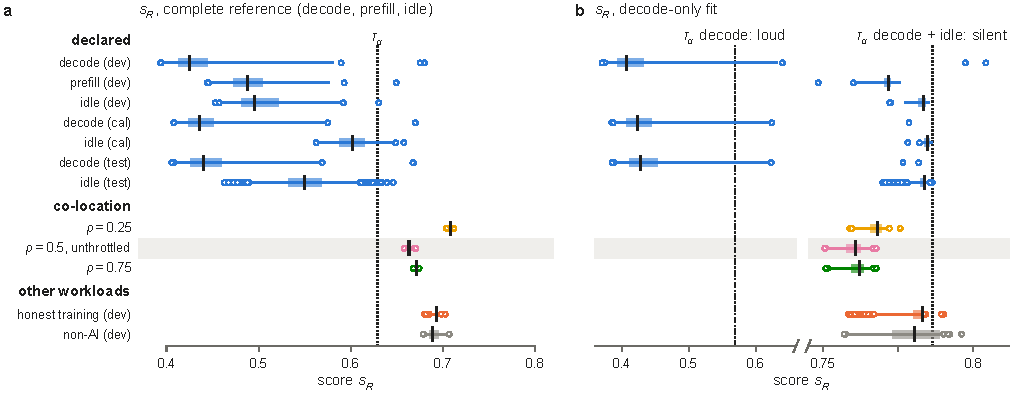
\includegraphics[width=\linewidth]{f7_r1.pdf}
  \caption{How $s_R$ scores each workload. Each row shows the per-window scores of one
    workload and split. Black ticks mark medians, bars the 25--75\% range and whiskers
    the 1--99\% range; circles are single windows beyond the whiskers. Windows to the right
    of $\tau_\alpha$ (dotted) are flagged. (a) The complete reference, with
    $\tau_\alpha = \TauRone$. It flags every co-location, honest-training and non-AI
    window. The shaded unthrottled run is the co-location run closest to $\tau_\alpha$; a
    few decode windows score above it (AUC \RoneAucDecode). (b) The decode-only fit
    (\cref{t:t7}), on a score axis broken at the slashes and widened beyond them. Prefill
    and idle are outside this fit, and idle now scores high. With idle in the threshold
    set, $\tau_\alpha = \TauDecOnlyPooled$ and no co-location window is flagged. With
    decode alone in it, $\tau_\alpha = \TauDecOnlyDecode$ and every co-location window
    and every idle window is flagged. Each threshold is labelled by its failure, as in
    \cref{t:t7}.}
  \label{f:f7}
\end{figure}

\paragraph{Training in the threshold set.} We add $k$ honest-training windows to the
\EthreeCalWindows{} calibration windows, with the fit unchanged. Detection of the
unthrottled run falls to zero at $k = \EthreeKOne$ to \EthreeKTen{} for $\alpha$
from 1\% to 10\%, and at $k = \EthreeKFive$ for $\alpha = \AlphaPct\%$. At that $k$, honest
training is still flagged at $\ge \EthreeHonestMin\%$; it falls as $k$ grows further
(\cref{f:f9}a).

\paragraph{Training in the fit.} We add $k$ development honest-training windows, drawn at
random, to the \EfourNDeclared{} declared windows of the fit, with the threshold set
unchanged. At $k = \EfourKHonest$ (\EfourShareHonest\% of the fit), the calibration-day
full fine-tuning run, which is outside every fit, is flagged at \EfourFullCal\%, while
LoRA stays at \EfourLoraCal\%. The median detection of the unthrottled run is
\EfourHalfDet\% at $k = \EfourKHalf$ and \EfourGoneDet\% at $k = \EfourKGone$
(\EfourShareGone\% of the fit). The declared windows of the fit are flagged at
\EfourDeclZero\% with a clean fit, and at \EfourDeclEnd\% at the largest $k$ (median over
draws; \cref{f:f9}b). These windows are in every fit, so the rate is in-sample.

\section{The cross-check on the corpus of Gargiulo and Kulp}\label{a:gk}

We fetched their \GkNTraces{} traces \citep{gkdataset} at a pinned revision, checked each file's hash,
and resampled from \GkRate{}~MS/s to \GkDecimated{}~kS/s with an exact rational
resampler and its anti-alias filter. We extracted our \NFeat{} features and fitted
their two forests: genuine, on their training, inference and non-AI traces; hardened,
adding their adversarial traces.

On their own traces, under their grouped five-fold protocol, our measurement chain reaches
macro-$F_1$ \GkOwnFone{} (range \GkOwnFoneLo{} to \GkOwnFoneHi) and accuracy
\GkOwnAcc. They report \GkFone{} and \GkAcc{} with \GkNFeat{} features at the full
rate. We did not reach their accuracy, and scored our windows anyway. Shuffled labels give \GkShuffle. Their traces pass an anti-alias
filter on decimation and ours do not, so features above about \GkAliasKhz{}~kHz differ
between the datasets.

\paragraph{The published hardened forest.}
\citet{gargiulo2026} harden their forest on four evasion strategies of their own. We
scored our windows with both forests (\cref{t:t5}). At their default threshold of
\DefaultDecision, their genuine forest misses the
unthrottled run ($\GkGenMiss\%$). Their hardened forest catches all three
co-location runs, but it also flags \GkHardPrefill\% of declared prefill windows as
training. Their hardening works here. Its cost falls on a declared workload that our
calibration day does not hold.

\begin{table}[!htbp]
  \centering
  \small
  % generated by scripts/table_t5.py from results/gk/t5.json (repo_commit 4494926)
% percent of windows flagged training; co-location over windows with >= 1 complete step
\begin{tabular}{lrr}
\toprule
Our windows & G\&K hardened & G\&K genuine \\
\midrule
honest training ($\geq 80$\%) & 100.0 & 100.0 \\
declared decode & 0.0 & 0.0 \\
declared prefill & 100.0 & 2.4 \\
declared, decode + prefill ($\leq 20$\%) & 16.7 & 0.4 \\
\midrule
co-location, $\rho = 0.25$ & 100.0 & 100.0 \\
co-location, $\rho = 0.5$ & 100.0 & 0.0 \\
co-location, $\rho = 0.75$ & 100.0 & 100.0 \\
\bottomrule
\end{tabular}

  \caption{Forests fitted by the recipe of \citet{gargiulo2026} (G\&K) on their corpus,
    scored on our windows: percent flagged training. The first rows are a
    transfer gate (training $\geq$ \GateTrain\%, declared
    $\leq$ \GateInf\%). Both forests pass. The hardened forest passes the declared
    row only because decode outnumbers prefill. Their chain and ours differ in rate
    and anti-alias filtering, and their own-data check fell short of their reported
    accuracy (\cref{a:gk}).}
  \label{t:t5}
\end{table}
